\section{Referencia de la Estructura symbol}
\label{structsymbol}\index{symbol@{symbol}}
Nodo de la tabla de simbolos.  


{\tt \#include $<$symtab.h$>$}

Diagrama de colaboraci\'{o}n para symbol:\begin{figure}[H]
\begin{center}
\leavevmode
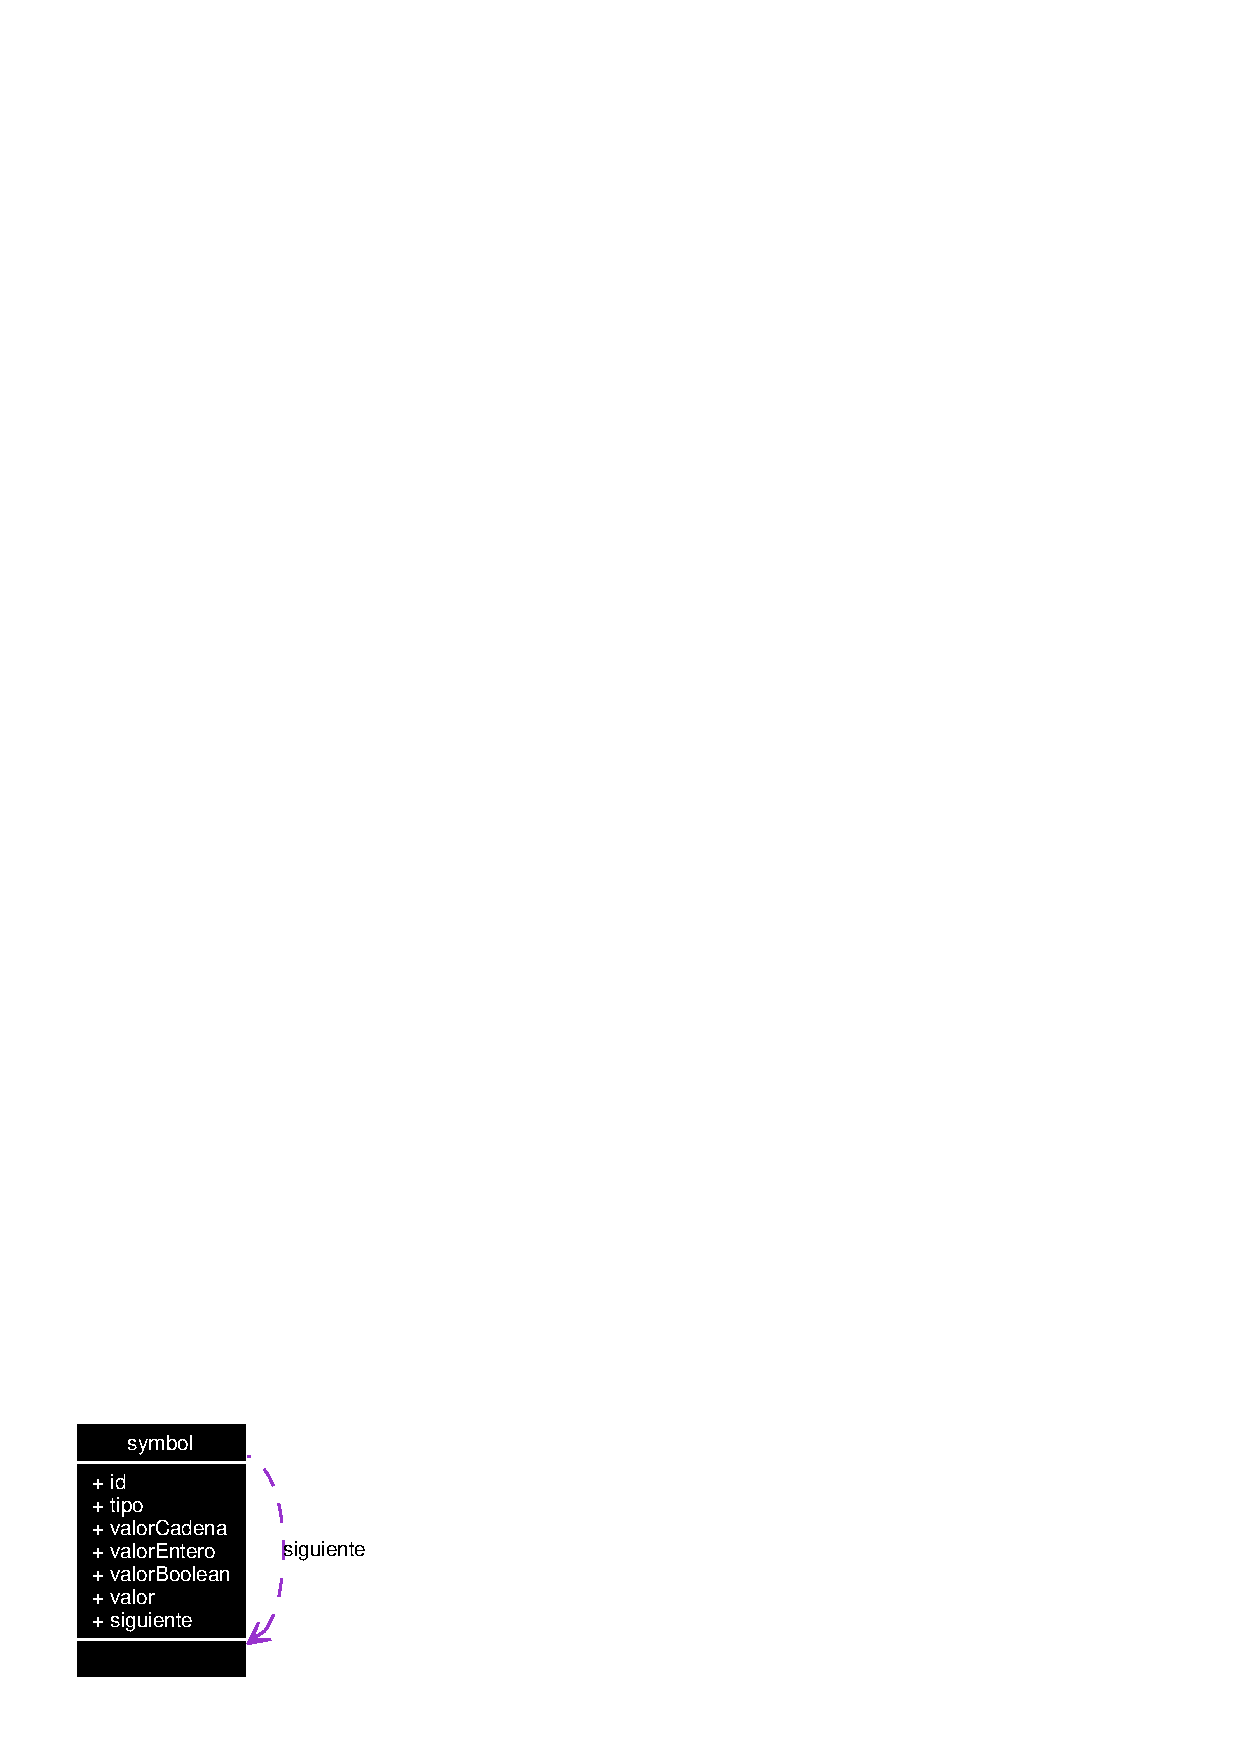
\includegraphics[width=88pt]{structsymbol__coll__graph}
\end{center}
\end{figure}
\subsection*{Atributos p\'{u}blicos}
\begin{CompactItemize}
\item 
char $\ast$ {\bf id}
\item 
int {\bf tipo}
\item 
\begin{tabbing}
xx\=xx\=xx\=xx\=xx\=xx\=xx\=xx\=xx\=\kill
union \{\\
\>char $\ast$ {\bf valorCadena}\\
\>int {\bf valorEntero}\\
\>char {\bf valorBoolean}\\
\} {\bf valor}\\

\end{tabbing}\item 
{\bf symbol} $\ast$ {\bf siguiente}
\end{CompactItemize}


\subsection{Descripci\'{o}n detallada}
Nodo de la tabla de simbolos. 



Definici\'{o}n en la l\'{\i}nea 13 del archivo symtab.h.

\subsection{Documentaci\'{o}n de los datos miembro}
\index{symbol@{symbol}!id@{id}}
\index{id@{id}!symbol@{symbol}}
\subsubsection{\setlength{\rightskip}{0pt plus 5cm}char$\ast$ {\bf symbol::id}}\label{structsymbol_o0}




Definici\'{o}n en la l\'{\i}nea 14 del archivo symtab.h.

Referenciado por borrar\-Nodos(), insertar\-Simbolo(), y print\-Symtab\-File().\index{symbol@{symbol}!siguiente@{siguiente}}
\index{siguiente@{siguiente}!symbol@{symbol}}
\subsubsection{\setlength{\rightskip}{0pt plus 5cm}{\bf symbol}$\ast$ {\bf symbol::siguiente}}\label{structsymbol_o6}




Definici\'{o}n en la l\'{\i}nea 21 del archivo symtab.h.

Referenciado por borrar\-Nodos(), buscar\-Simbolo(), insertar\-Simbolo(), y print\-Symtab\-File().\index{symbol@{symbol}!tipo@{tipo}}
\index{tipo@{tipo}!symbol@{symbol}}
\subsubsection{\setlength{\rightskip}{0pt plus 5cm}int {\bf symbol::tipo}}\label{structsymbol_o1}




Definici\'{o}n en la l\'{\i}nea 15 del archivo symtab.h.

Referenciado por borrar\-Nodos(), evaluar\-Asignacion(), evaluar\-Expresion(), evaluar\-For(), imprimir\-Tokens(), insertar\-Simbolo(), y print\-Symtab\-File().\index{symbol@{symbol}!valor@{valor}}
\index{valor@{valor}!symbol@{symbol}}
\subsubsection{\setlength{\rightskip}{0pt plus 5cm}union \{ ... \}  {\bf symbol::valor}}\label{structsymbol_o5}




Referenciado por borrar\-Nodos(), evaluar\-Asignacion(), evaluar\-Expresion(), evaluar\-For(), imprimir\-Tokens(), insertar\-Simbolo(), y print\-Symtab\-File().\index{symbol@{symbol}!valorBoolean@{valorBoolean}}
\index{valorBoolean@{valorBoolean}!symbol@{symbol}}
\subsubsection{\setlength{\rightskip}{0pt plus 5cm}char {\bf symbol::valor\-Boolean}}\label{structsymbol_o4}




Definici\'{o}n en la l\'{\i}nea 19 del archivo symtab.h.\index{symbol@{symbol}!valorCadena@{valorCadena}}
\index{valorCadena@{valorCadena}!symbol@{symbol}}
\subsubsection{\setlength{\rightskip}{0pt plus 5cm}char$\ast$ {\bf symbol::valor\-Cadena}}\label{structsymbol_o2}




Definici\'{o}n en la l\'{\i}nea 17 del archivo symtab.h.\index{symbol@{symbol}!valorEntero@{valorEntero}}
\index{valorEntero@{valorEntero}!symbol@{symbol}}
\subsubsection{\setlength{\rightskip}{0pt plus 5cm}int {\bf symbol::valor\-Entero}}\label{structsymbol_o3}




Definici\'{o}n en la l\'{\i}nea 18 del archivo symtab.h.

La documentaci\'{o}n para esta estructura fu\'{e} generada a partir del siguiente archivo:\begin{CompactItemize}
\item 
/media/docs/progra/c++/compiladores1/proy2/godzilla/src/{\bf symtab.h}\end{CompactItemize}
